% Chapter 4: Positivity in Equivariant Quantum Schubert Calculus
% 基于 Leonardo Constantin Mihalcea (约 2007)
% arXiv: alg-geom/0606006

\chapter{Positivity in Equivariant Quantum Schubert Calculus}
\label{chap:EquivariantQuantumPositivity}

\section{引言：从经典到量子——为什么要推广？}
\label{sec:FromClassicalToQuantum}

在前三章中，我们逐步建立了 Schubert calculus 的现代框架：\cref{chap:TriplePositivity} 在三重变量集下建立了 Graham positivity（\cref{def:GrahamPositivity}），\cref{chap:MolevSagan} 给出了 Molev-Sagan 类型公式，\cref{chap:QuantumDouble} 引入了量子双重 Schubert 多项式。每一步推广都自然地引出了下一个问题。

现在，一个自然的追问摆在我们面前：\textbf{经典上同调的正性能否推广到量子版本？}

这个问题并非无的放矢。我们已经知道，在经典等变上同调（equivariant cohomology）中，Graham 证明了 Peterson 的猜想（\cref{def:GrahamPositivity}）——展开系数是关于负根 $x_i$ 的非负多项式。但量子上同调的情况有所不同：乘法不再是单纯的相交计数，而涉及 Gromov-Witten 不变量（Gromov-Witten invariant）\footnote{问：什么是 Gromov-Witten 不变量？它计数的是什么？见附录 \cref{sec:GW-invariant}。}——计数的是满足特定条件的曲线个数。在更复杂的代数几何世界中，同类正性结果是否仍然成立？

\textbf{核心发现}（Mihalcea, 2007）：答案是肯定的。等变量子上同调（equivariant quantum cohomology）的结构常数 $c_{u,v}^{w,d}$ 仍然是关于负根 $x_1, \ldots, x_r$ 的非负整数系数多项式。

这个结果值得我们深思。通常，数学的每一次推广都会引入新的复杂性——更多的参数、更微妙的行为、更多的潜在反例。但在这里，Schubert calculus 的核心正性在从经典到量子的推广中表现出惊人的稳定性。这暗示着正性不仅仅是技术性的巧合，而是反映了某种更深层的几何和代数结构。

\section{历史脉络：Peterson 猜想}
\label{sec:PetersonConjectureHistory}

要理解 Mihalcea 的工作，需要回顾一段精彩的历史。这段历史展现了数学猜想如何通过一代代数学家的工作逐步得到证明和推广。

\subsection{经典情形}

在经典 Schubert calculus 中，结构常数 $c_{u,v}^w$ 计数旗流形中三个 Schubert 簇的交点个数，自然是非负整数。这种非负性（称为 \textbf{Schubert positivity}）植根于几何相交（geometric intersection）的具体计数——两条代数曲线在复流形中的相交个数 \cite[\S 1]{Chevalley1994}。

但当引入等变修正时，问题变得微妙了。等变上同调（equivariant cohomology）$H_T^*(G/P)$ 中的结构常数 $c_{u,v}^w$ 不再是简单的整数，而是关于 torus 作用参数的多项式 \cite{Borel1957,AndersonFulton}。\textbf{这些多项式的系数还能保持非负吗？}

这是一个深刻的问题。在等变量子上同调中，类不再是子簇的直接上同调类，而是提升到 $X \times_T ET$（同伦商空间，homotopy quotient）上的类。在这种更抽象的设置中，非负性不再能从几何相交直接读出。

\subsection{Peterson 的天才猜想}

1997 年，Daniel Peterson 在 MIT 的课堂上提出了一个令许多人惊讶的猜想：\textbf{即使在这些多项式中，系数仍然是``正''的}——具体而言，$c_{u,v}^w$ 可以写成负根 $-\alpha_i$ 的非负系数多项式。

为什么说这是``天才''的猜想？因为没有人能预期到这一点。等变量子上同调中的类失去了直接的几何意义，正性似乎不应该自动保持。Peterson 的洞察力在于他预见到了隐藏的统一结构。

这个猜想被 Graham 在 2001 年证明：

\begin{Theorem}[Graham Positivity Theorem {\cite[Theorem 3.2]{Gr}}]
\label{th:GrahamPositivity}
设 $X = G/P$ 为齐次空间，$u, v, w \in W^P$。则在等变上同调（equivariant cohomology）中，\footnote{问：$\sigma(u)^T$ 是什么意思？上标 $T$ 代表什么？见附录 \cref{sec:sigma-u-T}。}
$$\sigma(u)^T \cdot \sigma(v)^T = \sum_w c_{u,v}^w \sigma(w)^T$$
其中 $\sigma(u)^T$ 表示等变上同调（equivariant cohomology）中的 Schubert 类，$T$ 代表 torus 等变（equivariant）。\footnote{问：在 Schubert 演算中，$\sigma(w)$ 是什么意思？例如 $\sigma(1) = 1$（单位类）和 $\sigma(s_1) = [\text{点}]$（超平面类）。见附录 \cref{sec:SchubertClassSigma}。}
\end{Theorem}

\textbf{为什么叫``正性''？}\footnote{问：在 Graham Positivity 定理中，为什么说展开系数 $c^w_{u,v}(\mathbf{y}, \mathbf{t})$ 是 $t_j - y_i$ 的非负整数系数多项式？展开式中明明有负项（如 $-x_1t_2$）？见附录 \cref{sec:GrahamPositivityCoefficientMeaning}。} 因为每个 $c_{u,v}^w$ 都可以表示为形如 $x_1^{a_1} x_2^{a_2} \cdots$ 的单项式的非负线性组合，其中所有系数都是非负整数。

\subsection{量子化带来的挑战}

Graham 定理的证明利用了等变量子上同调的几何性质\footnote{问：在 Chapter 4 (Mihalcea) 中提到：``Graham 定理的证明利用了等变量子上同调的几何性质。``为什么 Graham 的证明要依赖几何性质？具体用了什么几何性质？到了量子上同调为何变得更复杂？见附录 \cref{sec:GrahamProofGeometry}。}。但当我们将目光投向量子上同调时，同样的正性问题变得更加复杂。在量子上同调（quantum cohomology）中，乘法不再是单纯的相交计数，而涉及 Gromov-Witten 不变量（Gromov-Witten invariant）\cite{Kontsevich1994,Gromov1985}——计数的是满足特定条件的曲线个数：

\begin{equation}
\sigma(u) \star \sigma(v) = \sum_{d} \sum_{w} q^d c_{u,v}^{w,d} \sigma(w).
\label{eq:QuantumProduct}
\end{equation}

这里 $d$ 是曲线类的多重次数（multi-degree），$q^d$ 是形式变量。\footnote{问：$\sigma(u) \star \sigma(v) = \sum_d \sum_w q^d c_{u,v}^{w,d} \sigma(w)$ 这个公式中，$q^d$ 是形式变量，$q$ 是什么？求和是对什么？$u, v, w$ 是什么？见附录 \cref{sec:q-formal-variable}。}关键问题出现了：系数 $c_{u,v}^{w,d}$ 作为 $x_i$ 的多项式，是否仍然满足正性？

一个自然的想法是：能否将量子情形``退化''到已知的 Graham 情形？如果能找到合适的极限或归约，Mihalcea 的工作正是基于这个思路。

\section{等变量子上同调的定义}
\label{sec:EQCDefinition}

在前一节中，我们看到了从经典到等变量子上同调的正性问题自然延伸。但等变量子上同调（equivariant quantum cohomology）究竟是什么？本节给出其正式定义。\footnote{问：$H^*(X \times_T ET)$ 是什么？是量子同调吗？$H^*(X \times_T ET)$ 是怎么定义的？我不了解上同调定义，这是量子同调吗？见附录 \cref{sec:EquivariantvsQuantum}。}

\subsection{思想来源：Kim 的贡献}

在深入定义之前，有必要提及 Kim 的重要贡献 \cite{Kim2000}。正是在 Kim 的工作基础上，Mihalcea 才得以将 Graham 的 positivity 结果推广到量子情形。Kim 认识到，等变上同调（equivariant cohomology）与量子上同调（quantum cohomology）之间存在一个``公共的母体''——等变量子上同调（equivariant quantum cohomology），它同时包含了这两者的结构 \cite[\S 1]{Kim2000}。

这一认识的关键在于：我们可以同时考虑 torus 作用（产生 $x_i$ 多项式）和量子修正（产生 $q$ 变量）。\footnote{问：这里 torus 作用为什么对应的是 $x_i$ 多项式？为什么量子修正产生 $q$ 变量？这个修正到底是什么含义？见附录 \cref{sec:torus-x-and-quantum-correction}。}

\subsection{设置}

以下 Setup 列出本文所需的核心几何对象。带 $\cref{chap:Intro}$ 引用的是 Chapter 1 中已有正式定义的概念；其余给出详细定义。

\begin{Definition}[\textbf{连通复半单李群}]\label{def:ConnectedComplexSemisimpleLieGroup}
$G$ 为\textbf{连通复半单李群}（connected complex semisimple Lie group）。这意味着：
\begin{enumerate}
\item $G$ 是复流形，同时带有光滑群结构；
\item 作为实流形，$G$ 是连通的；
\item 其李代数 $\mathfrak{g}$ 是半单（semisimple）的——即 $\mathfrak{g}$ 没有非平凡可解理想。
\end{enumerate}
典型例子：$\mathrm{GL}_n(\mathbb{C})$、$\mathrm{SL}_n(\mathbb{C})$、$\mathrm{Sp}_{2n}(\mathbb{C})$、$\mathrm{SO}_n(\mathbb{C})$ 等。
\end{Definition}

\begin{Definition}[\textbf{抛物子群}]\label{def:ParabolicSubgroup}
$P \subset G$ 为\textbf{抛物子群}（parabolic subgroup）。这等价于：存在一个 Borel 子群 $B \subset G$（极大连通可解子群）使得 $B \subset P$。几何上，$G/P$ 是紧齐次空间（compact homogeneous space），称为旗流形（flag variety）的推广。
\end{Definition}

\begin{Definition}[\textbf{Borel 子群与极大环面}]\label{def:BorelAndMaximalTorus}
$B \subset P$ 为\textbf{Borel 子群}（Borel subgroup），即 $G$ 的极大连通可解子群。$T \subset B$ 为\textbf{极大环面}（maximal torus），满足 $T \cong (\mathbb{C}^\times)^r$，其中 $r = \operatorname{rank}(G)$ 为 $G$ 的秩（rank）。$T$ 在 $G$ 的结构理论中扮演中心角色：它决定了根系统的几何。
\end{Definition}

\begin{Definition}[\textbf{齐次空间}]\label{def:HomogeneousSpace}
$X = G/P$ 为\textbf{齐次空间}（homogeneous space）。这意味着群 $G$ 通过左乘作用传递地作用在 $X$ 上，$P$ 为该作用的迷向子群（isotropy subgroup）。当 $P = B$ 时，$X = G/B$ 是旗流形（flag variety）；当 $P$ 对应 Grassmannian 型子群时，$X$ 是部分旗流形。
\end{Definition}

\begin{Definition}[\textbf{Weyl 群与 $W_P$ 子群}]\label{def:WeylGroupAndWP}
$W$ 为 $G$ 的\textbf{Weyl 群}（Weyl group），见 \cref{def:WeylGroup}（Chapter 1）。$W_P \subset W$ 为由 $P$ 确定的子群：它是 $W$ 中所有使 $\Delta_P$（见下）保持不变的 Weyl 反射生成的子群。\footnote{问：Weyl 群与 $W_P$ 子群的具体例子？例如 $GL_3$ 中不同抛物子群对应的 $W_P$ 是什么？见附录 \cref{sec:qa-WeylGroupAndWP}。}
\end{Definition}

\begin{Definition}[\textbf{正单根系与 $\Delta_P$}]\label{def:PositiveRootSystemAndDeltaP}
$\Delta = \{\alpha_1, \ldots, \alpha_r\}$ 为\textbf{正单根系}（positive simple root system），见 \cref{def:CartanRootSystem}（Chapter 1）。选取一个 Borel 子群 $B$ 对应一个正根的选择。$\Delta_P \subset \Delta$ 为由 $P$ 确定的子集：它是 $\Delta$ 中被 $P$（或等价地，被其对应的抛物子群）包含的简单根的集合。直观上，$\Delta_P$ 记录了 $P$ 在 Weyl 群中``忘记``了哪些反射方向。
\end{Definition}

\begin{Definition}[\textbf{最短长度代表元 $W^P$}]\label{def:ShortestLengthRepresentatives}
$W^P \subset W$ 为 $W/W_P$ 的\textbf{最短长度代表元集合}（shortest length representatives）。即：每个陪集 $wW_P \in W/W_P$ 中唯一的长度最短元素。形式化地，
$$W^P = \{w \in W \mid \ell(w) \leqslant \ell(w') \text{ 对所有 } w' \in wW_P\}$$
其中 $\ell(w)$ 是 Weyl 群的长度函数（$w$ 的 inversion 个数）。$W^P$ 在 Schubert 理论中扮演关键角色：$G/P$ 的 Schubert 细胞由 $W^P$ 参数化。
\end{Definition}

记 $\Lambda = H_T^*(pt) = \mathbb{Z}[x_1, \ldots, x_r]$\footnote{问：等变量子上同调类是如何定义的？见附录 \cref{sec:EquivariantCohomologyClass}。}，其中 $x_i$ 对应负单根 $-\alpha_i$（negative simple roots）。

\subsection{等变量子上同调}

基于 Kim 的思想，Mihalcea 将等变量子上同调定义为分次 $\Lambda[q]$-代数。

\begin{Definition}[\textbf{等变量子上同调}]
\label{def:EquivariantQuantumCohomology}
\textbf{等变量子上同调}（equivariant quantum cohomology）$QH_T^*(X)$ 是一个分次 $\Lambda[q]$-代数，其 $\Lambda[q]$-基底为 $\{\sigma(w) \mid w \in W^P\}$。乘法 $\circ$ 定义为：
\begin{equation}
\sigma(u) \circ \sigma(v) = \sum_{d} \sum_{w \in W^P} q^d c_{u,v}^{w,d} \sigma(w),\footnote{问：$\sigma(u) \circ \sigma(v) = \sum_{d} \sum_{w \in W^P} q^d c_{u,v}^{w,d} \sigma(w)$ 这个公式中，这两个求和分别是对什么求和的？见附录 \cref{sec:qa-eqc-summations}。}
\label{eq:EQCDefinition}
\end{equation}
其中 $c_{u,v}^{w,d}$ 称为\textbf{等变量子 Littlewood-Richardson 系数}（equivariant quantum LR coefficient，简称 Equivariant Quantum Littlewood-Richardson 系数）。\footnote{问：在 \cref{def:EquivariantQuantumCohomology} 中提到：$QH_T^*(X)$ 是一个分次 $\Lambda[q]$-代数。什么是分次 $\Lambda[q]$-代数？其中的 $q$ 变量代表什么？见附录 \cref{sec:graded-Lambda-q-algebra}。}
\end{Definition}

\textbf{关键性质}：$c_{u,v}^{w,d} \in \Lambda = \mathbb{Z}[x_1, \ldots, x_r]$ 是齐次多项式，次数为 $c(u) + c(v) - c(w) - \sum d_i \cdot \deg(q_i)$\footnote{问：次数公式 $c(u) + c(v) - c(w) - \sum d_i \cdot \deg(q_i)$ 中的求和指标 $i$ 的范围是什么？见附录 \cref{sec:qa-degree-summation-range}。}。

\textbf{与经典情形的关系}：等变量子上同调是以下两者的共同推广：
\begin{itemize}
\item 当 $d = 0$ 时，退化为等变上同调（equivariant cohomology）$H_T^*(X)$（对应 Graham positivity）\footnote{问：为什么当 $d = 0$ 时，量子乘积公式 $\sigma(u) \circ \sigma(v) = \sum_{d} \sum_{w} q^d c_{u,v}^{w,d} \sigma(w)$ 退化为等变上同调 $H_T^*(X)$（对应 Graham positivity）？见附录 \cref{sec:d-zero-degeneracy}。}；
\item 当所有 $x_i = 0$ 时，退化为普通量子上同调（quantum cohomology）$QH^*(X)$\footnote{问：为什么当 $x_i = 0$ 时，退化为普通量子上同调 $QH^*(X)$？这其中的数学机制是什么？见附录 \cref{sec:xi-zero-degeneracy}。}。
\end{itemize}

这种``共同推广''的性质解释了为什么等变量子上同调是一个自然的研究对象——它同时推广了两个重要的上同调理论。

\subsection{Kim 的结构定理}
\label{sec:KimStructureTheorem}

在前一节的定义之后，Kim 证明了等变量子上同调具有代数结构。\footnote{问：Kim 的等变量子上同调结构定理（Proposition 3.1）到底说了什么？证明在哪里？直观上如何理解两个同构？见附录 \cref{sec:KimStructureTheorem}。}

\begin{Theorem}[等变量子上同调的结构 {\cite[Proposition 3.1]{Kim2000}}]
\label{th:KimStructure}
设 $X = G/P$ 为齐次空间，则 $(A, \circ)$ 是交换、结合的 $\Lambda[q]$-代数，其中 $A = QH_T^*(X)$。进一步，有以下标准同构：
\begin{enumerate}
\item[(1)] $A / \langle \Lambda^{+} \cdot A \rangle \simeq QH^*(X)$ 作为 $\mathbb{Z}[q]$-代数；
\item[(2)] $A / \langle q \cdot A \rangle \simeq H_T^*(X)$ 作为 $\Lambda$-代数。
\end{enumerate}
其中 $\Lambda^{+} \subset \Lambda$ 表示由正次数元素构成的真理想。
\end{Theorem}

\textbf{意义解读}：这个命题告诉我们，等变量子上同调 $QH_T^*(X)$ 同时包含两个重要退化的代数结构：
\begin{itemize}
\item 第一个同构表明，当我们``忘掉'' $x_i$（即取 $\Lambda^{+}$ 理想商），只剩下量子参数 $q$，得到普通量子上同调 $QH^*(X)$；
\item 第二个同构表明，当我们``忘掉'' $q$（即取 $q$ 生成的理想商），只剩下 $x_i$ 参数，得到等变上同调 $H_T^*(X)$。
\end{itemize}

\textbf{为什么这个定理重要？}它证明了等变量子上同调的乘法确实良定义且满足交换律和结合律——这是 Mihalcea 整个 positivity 证明的基础。

\textbf{与 Equivariant Quantum Littlewood-Richardson 系数的关系}：由这些同构可以推出，当 $d = 0$ 时，$c_{u,v}^{w,d}$ 退化为等变 LR 系数 $c_{u,v}^w$；当 $c_{u,v}^{w,d}$ 的多项式次数为 0 时（即 $c(u) + c(v) = c(w) + \sum d_i \cdot \deg q_i$），它等于普通量子 LR 系数。

\subsection{例子}

\textbf{例 1：Grassmannian $Gr(1,2) = \mathbb{P}^1$ 的情形。}\footnote{问：请详细解释 $Gr(1,2) = \mathbb{P}^1$ 的例子，逐变量映射到一般公式，并验证其性质。请见附录 \cref{sec:Gr12-P1-example}。}

设 $X = Gr(1,2) = \mathbb{P}^1$。此时 $W = S_2 = \{1, s_1\}$，只有两个 Schubert 类：

\begin{itemize}
\item $\sigma(1) = 1$（单位类）；
\item $\sigma(s_1) = [\text{点}]$（超平面类，记作 $H$）。
\end{itemize}

等变量子上同调 $QH_T^*(\mathbb{P}^1)$ 的乘法为：
$$\sigma(s_1) \circ \sigma(s_1) = q \sigma(1).\footnote{问：为什么在量子乘积公式 $\sigma(s_1) \circ \sigma(s_1) = q \sigma(1)$ 中，$w = s_1$ 不可能出现，而只能是 $w = 1$？见附录 \cref{sec:qa-w-s1-degree-mismatch}。}$$

\textbf{几何意义}：$\mathbb{P}^1$ 上两点决定的直线与自身的交点数为 1，但需要量子修正因子 $q$（计数亏格 0 曲线）。\footnote{问：为什么 $c_{s_1,s_1}^{1,1} = 1$？这个量子修正系数背后的数学机制是什么？见附录 \cref{sec:QuantumCorrectionCoefficients}。}

\textbf{例 2：$Gr(2,4)$ 情形。}\footnote{问：请详细解释 Mihalcea 论文中关于 $Gr(2,4)$ 的例子（chapter4.tex 第 143-156 行），用最简单的语言说明：1. $Gr(2,4)$ 是什么？为什么叫 Grassmannian？2. $W = S_4$ 是什么？最短代表元是什么意思？为什么有 6 个？3. $u = s_1$, $v = s_3$ 是什么？$\sigma$ 是什么？4. 乘积 $\sigma(s_1) \circ \sigma(s_3)$ 是什么意思？5. 右边两项 $\sigma(s_1 s_3)$ 和 $(x_2 - x_3) q \sigma(1)$ 各自代表什么几何意义？6. 为什么要验证 $x_2 - x_3$ 是``非负系数``？这为什么重要？7. 量子修正项 $(x_2 - x_3) q \sigma(1)$ 中的 $q$ 是什么？$q$ 记录曲线的同调类是什么意思？请见附录 \cref{sec:qa-gr24}。}

设 $X = Gr(2,4)$（2 维平面构成的 Grassmannian）。此时 $W = S_4$ 的最短代表元有 6 个，对应 6 个 Schubert 类。

考虑 $u = s_1$，$v = s_3$。在等变量子上同调中：
$$\sigma(s_1) \circ \sigma(s_3) = \sigma(s_1 s_3) + (x_2 - x_3) q \sigma(1).$$

\textbf{正性验证}：这里 $x_2 - x_3$ 是非负系数多项式（系数为 1），体现了 Mihalcea positivity 的核心结论。这正是我们在 \cref{th:EQCPositivity} 中要证明的性质——Equivariant Quantum Littlewood-Richardson 系数是关于负根 $x_i$ 的非负整数系数多项式。

其中：
\begin{itemize}
\item $\sigma(s_1 s_3)$ 是普通项（对应 $d = 0$）；
\item $(x_2 - x_3) q \sigma(1)$ 是量子修正项，其中 $x_2 - x_3$ 是非负系数多项式（体现正性！），$q$ 记录曲线的同调类。
\end{itemize}

\textbf{例 3：退化情形。}

检验正性：
\begin{itemize}
\item 当 $d = 0$ 时，$c_{u,v}^{w,0}$ 退化为 Graham 情形——非负系数多项式；
\item 当 $x_i = 0$ 时，$c_{u,v}^{w,d}$ 退化为普通量子系数——非负整数。
\end{itemize}

这验证了 \cref{def:EquivariantQuantumCohomology} 中的退化关系。

\section{主要定理}
\label{sec:MainTheoremCh4}

现在我们可以陈述 Mihalcea 的核心结果。这个定理回答了我们在引言中提出的问题。

\begin{Theorem}[等变量子上同调 Positivity {\cite[Theorem 1]{Mihalcea}}]
\label{th:EQCPositivity}
设 $u, v, w \in W^P$ 且 $d$ 为多重次数。则等变量子 Littlewood-Richardson 系数 $c_{u,v}^{w,d}$ 是关于负根 $x_1, \ldots, x_r$ 的非负整数系数多项式。
\end{Theorem}

这个定理的证明策略本身就是一段精彩的故事——Mihalcea 发现，可以将量子情形的计算归约到已经解决的 Graham 情形。我们将在下一节详细讨论这个证明思路。

\subsection{正性概念的演进}

为了理解这个定理的意义，让我们比较一下不同层次的正性：

\begin{center}
\begin{tabular}{c|c|c}
情形 & 退化为 & 正性 \\ \hline
经典上同调 & $c_{u,v}^w \in \mathbb{N}$ & 非负整数 \\
等变量子上同调 & $c_{u,v}^w \in \mathbb{Z}[x_i]$ & 非负系数多项式 \\
等变量子上同调（带量子修正） & $c_{u,v}^{w,d} \in \mathbb{Z}[x_i]$ & 非负系数多项式
\end{tabular}
\end{center}

\textbf{核心洞察}：从经典到量子，正性性质一直保持——量子变量 $q$ 的引入并不破坏正性。这与量子化往往引入负号或其他复杂行为的直觉相反。更重要的是，每一代的正性都包含了前一代作为特殊情形（取特定的退化参数）：
$$c_{u,v}^w \in \mathbb{N} \Longrightarrow c_{u,v}^w \in \mathbb{Z}[x_i] \Longrightarrow c_{u,v}^{w,d} \in \mathbb{Z}[x_i].$$

这暗示着正性不仅仅是技术性的巧合，而是反映了 Schubert calculus 深层的不变结构。

\subsubsection{三种正性定理的正式陈述与符号溯源}

为了清晰理解三者关系，我们逐一给出完整的乘法公式。\footnote{问：经典 Schubert 乘法、 Graham 正性、 Mihalcea 正性三者公式形式上有什么共同点和区别？分别写出它们的完整乘法公式。见 \S\ref{sec:MainTheoremCh4}。}

\smallskip
\noindent\textbf{定理一：经典 Schubert Positivity（几何相交版本）}

\begin{Theorem}[Schubert Positivity — 几何版本]
\label{th:ClassicalSchubertPositivity}
在普通上同调 $H^*(G/P)$ 中，Schubert 胞腔类满足乘法
\begin{equation}
\label{eq:ClassicalSchubertProduct}
\sigma(u) \cdot \sigma(v) = \sum_{w \in W^P} c_{u,v}^w \, \sigma(w),
\end{equation}
其中结构常数 $c_{u,v}^w \in \mathbb{N}$ 是非负整数，等于三个 Schubert 簇 $X(u), X(v), X(w^\perp)$ 在旗流形中的一般位置相交点数。
\end{Theorem}

\smallskip
\noindent\textbf{定理二：Graham Positivity（等变上同调版本）}

\begin{Theorem}[Graham Positivity — 等变上同调版本 {\cite[ Theorem 3.2]{Gr}}]
\label{th:GrahamPositivityCh4}
在等变上同调 $H_T^*(G/P)$ 中，Schubert 类满足乘法
\begin{equation}
\label{eq:GrahamProduct}
\sigma^T(u) \cdot \sigma^T(v) = \sum_{w \in W^P} c_{u,v}^w(\mathbf{x}) \, \sigma^T(w),
\end{equation}
其中结构常数 $c_{u,v}^w(\mathbf{x}) \in \mathbb{Z}[x_1,\ldots,x_r]$ 是关于 torus 权 $x_i$（即负根 $-\alpha_i$）的非负整数系数多项式。\footnote{问：Graham 正性中的 $c_{u,v}^w(\mathbf{x})$ 和第一章 Graham 公式中的 $c^w_{u,v}(\mathbf{y},\mathbf{t}) \in \mathbb{Z}_\geq0[t_i - y_j]$ 有什么关系？见 \S\ref{sec:MainTheoremCh4} 的比较表。}
\end{Theorem}

\smallskip
\noindent\textbf{定理三：Mihalcea Positivity（等变量子量子版本）}

\begin{Theorem}[Mihalcea Positivity — 等变量子量子 cohomology 版本 {\cite[ Theorem 1]{Mihalcea}}]
\label{th:MihalceaPositivityCh4}
在等变量子量子上同调 $QH_T^*(G/P)$ 中，Schubert 类满足乘法
\begin{equation}
\label{eq:MihalceaProduct}
\sigma^T(u) \star \sigma^T(v) = \sum_{w,d} q^d \, c_{u,v}^{w,d}(\mathbf{x}) \, \sigma^T(w),
\end{equation}
其中 $d \in \mathbb{N}^r$ 是多重次数（degree），$q^d$ 是形式量子变量，结构常数 $c_{u,v}^{w,d}(\mathbf{x}) \in \mathbb{Z}[x_1,\ldots,x_r]$ 是非负整数系数的多项式。
\end{Theorem}

\smallskip
\noindent\textbf{三者退化关系与符号对应}：\footnote{问：$x_i$、$y_j$、$t_k$ 三种符号体系分别出现在哪些公式中？它们之间的对应关系是什么？见 \S\ref{sec:MainTheoremCh4} 的比较表。}

\begin{center}
\begin{tabular}{p{2.5cm}|p{3cm}|p{4cm}|p{4.5cm}}
\hline
\textbf{正性定理} & \textbf{上同调层次} & \textbf{结构常数} & \textbf{变量环} \\ \hline
Schubert（定理一） & 普通 $H^*(G/P)$ & $c_{u,v}^w \in \mathbb{N}$ & 无参数 \\ \hline
Graham（定理二） & 等变 $H_T^*(G/P)$ & $c_{u,v}^w(\mathbf{x}) \in \mathbb{Z}[x_i]$ & $x_i$：torus 权 / 负根 \\ \hline
Mihalcea（定理三） & 量子 $QH_T^*(G/P)$ & $c_{u,v}^{w,d}(\mathbf{x}) \in \mathbb{Z}[x_i]$ & $x_i$ 同上，$q^d$：量子修正 \\ \hline
双重 Graham（二重 $\mathbf{S}_w$） & 等变 $H_T^*(G/P)$（双变量） & $c_{u,v}^w(\mathbf{y},\mathbf{t}) \in \mathbb{Z}[t_i - y_j]$ & $\mathbf{y}, \mathbf{t}$：两组 torus 权 \\ \hline
\end{tabular}
\end{center}

关键符号对应关系：
\begin{itemize}
\item $x_i$（ch4）$= -\alpha_i$（torus 权 = 负根），对应第一章中的 $t_i - y_j$ 当 $y_j$ 取特定值时
\item \eqref{eq:GrahamProduct} 中的 $c_{u,v}^w(\mathbf{x})$ 与 \cref{def:GrahamPositivity} 中的 $c^w_{u,v}(\mathbf{y},\mathbf{t})$ 是同一常数在不同变量系下的表示
\item \eqref{eq:ClassicalSchubertProduct} 是 \eqref{eq:GrahamProduct} 在 $x_i \to 0$（忘掉 torus 作用）的退化
\item \eqref{eq:MihalceaProduct} 是 \eqref{eq:GrahamProduct} 加入量子修正 $q^d$ 的推广
\item 双重 Graham（\cref{def:GrahamPositivity}）是两变量情形 $c_{u,v}^w(\mathbf{y},\mathbf{t})$：$\mathbf{y}$ 记录左作用位移，$\mathbf{t}$ 记录右作用位移，$\mathbf{S}_u(\mathbf{x};\mathbf{y}) \cdot \mathbf{S}_v(\mathbf{x};\mathbf{t}) = \sum_w c_{u,v}^w(\mathbf{y},\mathbf{t}) \mathbf{S}_w(\mathbf{x};\mathbf{t})$
\end{itemize}

这暗示着正性不仅仅是技术性的巧合，而是反映了 Schubert calculus 深层的不变结构——无论从几何相交（古典）、等变上同调（Graham）、还是量子上同调（Mihalcea）切入，本质都是 Schubert 胞腔相交计数的非负性。

\section{证明思路：归约到 Graham 定理}
\label{sec:ProofOutlineCh4}

Mihalcea 的证明思路巧妙而简洁。核心思想是：将 Equivariant Quantum Littlewood-Richardson 系数的计算归约到已在 Graham 定理中解决的问题。

\textbf{论文的核心——§6 证明结构}（\cite[§6, 第8-11页]{Mihalcea}）：Mihalcea 的论文 \S 6（第8-11页）包含了 positivity 定理的完整证明。整个证明的灵魂是\textbf{归约思想}：将 Equivariant Quantum Littlewood-Richardson 系数计算归约到已知的 Graham positivity。

证明分为两部分：

\textbf{（1）§6.1 准备工作——两个核心要素}：
\begin{itemize}
\item 在 $X \times X$ 上定义半直积 $B' = T \cdot (U^- \times U^-)$ 的作用
\item 通过投影公式，将 $\overline{\mathcal{M}}_{0,3}(X,d)$ 上的曲线计数问题归约到 $X \times X$
\end{itemize}

\textbf{（2）§6.2 定理证明——三层逻辑链}：

\begin{itemize}
\item \textbf{Lemma 6.4}（\cref{prop:ev3inverse}，\cite[Lemma 6.4]{Mihalcea}）：$ev_3^{-1}(Y(w))$ 的不可约分支
\item \textbf{Corollary 6.2}（\cref{cor:GrahamOnXX}，\cite[Corollary 6.2]{Mihalcea}）：$X \times X$ 上的 Graham Positivity
\item \textbf{Lemma 6.3}（\cref{prop:KleimanTransversality}，\cite[Lemma 6.3]{Mihalcea}）：Kleiman transversality：$F: Z \to X \times X$ 是 $G$-等变映射，则 $F^{-1}(X(u) \times Y(v))$ 是 reduced、locally irreducible，余维数为 $c(u) + l(v)$
\end{itemize}

\textbf{证明的关键步骤}：先用 \cref{prop:ev3inverse} 将 $ev_3^{-1}(Y(w))$ 分解为不可约分支 $V_i$，再用 \cref{prop:KleimanTransversality}（Kleiman transversality）处理每个 $V_i$ 通过 $F = (ev_1, ev_3)$ 在 $X \times X$ 上的像，最后由 \cref{cor:GrahamOnXX}（Graham Positivity）保证每个 $[F(V_i)]_T$ 都是非负组合。投影公式则将这些结果``推送''回 $\overline{\mathcal{M}}_{0,3}(X,d)$ 上的 Equivariant Quantum Littlewood-Richardson 系数。

\textbf{Lemma 6.3 的正式陈述}（\cite[Lemma 7.2]{FW}，见 \cref{prop:KleimanTransversality}）：设 $Z$ 是不可约 $G$-簇，$F: Z \to X \times X$ 是 $G$-等变映射（$G$ 在 $X \times X$ 上对角作用）。则对任意 $u, v \in W^P$，$F^{-1}(X(u) \times Y(v))$ 是 reduced、locally irreducible 的，其余维数为 $c(u) + l(v)$。

整个证明的灵魂是 \textbf{归约思想}：通过投影公式，将 $\overline{\mathcal{M}}_{0,3}(X,d)$\footnote{问：$\overline{\mathcal{M}}_{0,3}(X,d)$ 是什么？每个符号的含义是什么？为什么要有紧化？什么是评估映射 $ev_i$？能举一个 $\mathrm{Gr}(2,4)$ 的具体例子吗？见附录 \cref{sec:MOD-space}。} 上的曲线计数问题归约到 $X \times X$ 上的已知正性。\footnote{等变量子上同调 positivity 定理的完整证明见附录 \cref{sec:appendix-eqc-proof}。}

\subsection{为什么可以归约？}

在证明之前，让我们理解这个策略的直觉。Equivariant Quantum Littlewood-Richardson 系数涉及稳定映射模空间 $\overline{\mathcal{M}}_{0,3}(X,d)$——它参数化了满足特定条件的稳定映射 $f: \mathbb{P}^1 \to X$\footnote{问：在量子上同调的定义中，出现稳定映射 $f: \mathbb{P}^1 \to X$，这里的 $X$ 是什么？$\mathbb{P}^1$ 又是什么？见附录 \cref{sec:P1-to-X}。}。

但 Mihalcea 的关键洞察是：\textbf{通过投影公式，复杂的上同调表达式可以``推送''到 $X \times X$ 上，而 Graham positivity 已经告诉我们答案。}

这个策略类似于我们在微积分中处理复杂积分时使用的变量替换——将一个难以处理的问题转化到我们已经理解的框架中。

这一归约策略与 \cref{chap:TriplePositivity} 中 Gao-Xiong 证明三重 Schubert positivity 的思路有本质联系——两者都使用了\textbf{投影公式}（projection formula）将复杂的几何对象分解为已知的组成部分 \cite[Section 3]{GX2025}。

\subsection{核心工具：投影公式与推送公式}

在深入证明之前，我们需要了解两个关键的代数几何工具。

\subsubsection{投影公式（Projection Formula）}

设 $f: X_1 \to X_2$ 为 $T$-等变映射。对于
$a \in H_T^*(X_2)$、$b \in H_T^*(X_1)$，有：
\begin{equation}
f_*^T\left((f^T)^*(a) \cdot b\right) = a \cdot f_*^T(b).
\label{eq:ProjectionFormulaCh4}
\end{equation}

\textbf{直观理解}：想象你有两个房间 $X_1$ 和 $X_2$，中间有一扇门（映射 $f$）。现在你站在 $X_2$ 里有一张纸条 $a$，在 $X_1$ 里有一张组合纸条 $b$。如果你想把 $X_1$ 里所有东西都搬到 $X_2$，那么纸条 $b$ 上那些``来自 $X_2$ 的部分``（即 $(f^T)^*(a)$）会在搬运过程中保持不变，只需要对 $b$ 的其余部分做推送。这个公式就是说：\textbf{来自目标空间的类 $a$ 在推送过程中可以``穿过``整个运算，单独留在外面}。

\textbf{为什么这很有用？}：在量子上同调的证明中，我们需要计算
$$c_{u,v}^{w,d} = \pi_*^T\left((ev_1^T)^* \sigma(u)^T \cdot (ev_2^T)^* \sigma(v)^T \cdot (ev_3^T)^* \widetilde{\sigma}(w)^T\right).$$
这里 $\sigma(u)^T$ 和 $\sigma(v)^T$ 是来自旗流形 $X$ 的类，而 $ev_1, ev_2$ 是从模空间 $\overline{\mathcal{M}}$ 到 $X$ 的映射。通过投影公式，我们可以把来自 $X$ 的因子``提取``出来，只对复杂的模空间部分做推送——这就是从 $\overline{\mathcal{M}}$ 转移到 $X \times X$ 的关键。

\textbf{生活中的类比}：想象你在整理行李。你有一个大箱子 $X_1$（模空间 $\overline{\mathcal{M}}$），要把它所有东西都转移到小箱子 $X_2$（积空间 $X \times X$）。你知道有些东西（$a$）本来就是从 $X_2$ 带来的，所以它们在转移后还是一样。而那些真正属于 $X_1$ 的东西（$b$）则需要被``压缩``或``重新打包``。投影公式就是描述这个打包规则的数学语言。

投影公式在 \cref{chap:TriplePositivity} 的证明中也扮演了核心角色——它建立了从几何相交到上同调类的桥梁 \cite[Lemma 2.5]{AndersonFulton}。

\subsubsection{推送公式（Push-Forward Formula）}

对于纤维积图（fiber product diagram），有：
\begin{equation}
f_*([V]) = \sum_i m_i a_i [f(V_i)],
\label{eq:PushForwardCh4}
\end{equation}
其中 $V_i$ 是原像的不可约分支（irreducible component），$m_i$ 是对应的次数。

这个公式允许我们将一个复杂子簇的推送分解为其各个不可约分支的推送的线性组合。

\subsection{第一步：在 $X \times X$ 上工作}

考虑积空间 $X \times X$，带有半直积 $B' = T \cdot (U^- \times U^-)$ 的作用：
$$t \cdot (u_1, u_2)(\bar{g}_1, \bar{g}_2) = (tu_1\bar{g}_1, tu_2\bar{g}_2).$$

选择这个特定的 torus 作用是精心设计的——它让我们能够利用 $X \times X$ 上的特殊几何性质。

\textbf{关键引理}（\cite[Corollary 6.2]{Mihalcea}）：

\begin{Lemma}[Graham Positivity on $X \times X$]
\label{lem:GrahamOnProductXtimesX}
设 $V \subset X \times X$ 为 $T$-稳定子簇（$T$-stable subvariety）。则在 $H_T^*(X \times X)$ 中，
$$[V]_T = \sum_i f_i [Y(u_i) \times Y(v_i)]_T,$$
其中每个 $f_i \in \Lambda = \mathbb{Z}[x_1, \ldots, x_r]$ 是非负系数多项式。
\end{Lemma}

这意味着任何 $T$-稳定子簇在上同调中都可以写成 $Y(u) \times Y(v)$ 型的类的非负线性组合。这是 Graham 定理在乘积空间上的自然应用。

\subsection{第二步：使用 Projection Formula}

设 $\overline{\mathcal{M}} = \overline{\mathcal{M}}_{0,3}(X,d)$ 为稳定映射的模空间（stable map moduli space），$ev_i : \overline{\mathcal{M}} \to X$ 为评估映射（evaluation map）。

\leavevmode\newline\textbf{Equivariant Quantum Littlewood-Richardson} 系数定义为：
$$c_{u,v}^{w,d} = \pi_*^T\left((ev_1^T)^* \sigma(u)^T \cdot (ev_2^T)^* \sigma(v)^T \cdot (ev_3^T)^* \widetilde{\sigma}(w)^T\right).$$

考虑映射 $F = (ev_1, ev_2)$，
以及映射 $\overline{\mathcal{M}} \to X \times X$，
它将模空间投影到前两标记点的积空间上。

利用投影与推送公式，Mihalcea 将表达式转化为：
$$c_{u,v}^{w,d} = \sum_i a_i (\pi_{X \times X})_*^T\left([X(u) \times X(v)]_T \cdot [F(V_i)]_T\right),$$
其中 $V_i$ 是 $ev_3^{-1}(Y(w))$ 的不可约分支（irreducible component），由 \cite[Lemma 6.4]{Mihalcea} 给出。

\textbf{这一步的关键}：我们成功地将问题从 $\overline{\mathcal{M}}$ 转移到了 $X \times X$。

\subsection{第三步：应用 Graham 定理}

对每个 $F(V_i)$，由 Lemma \cref{lem:GrahamOnProductXtimesX}，我们可以写
$$[F(V_i)]_T = \sum_j f_j^i [Y(u_j) \times Y(v_j)]_T.$$

代入并再次使用投影公式，得到
$$(\pi_{X \times X})_*^T\left([X(u) \times X(v)]_T \cdot [Y(u_j) \times Y(v_j)]_T\right) = \delta_{u,u_j} \cdot \delta_{v,v_j},$$
其中 $\delta$ 为 Kronecker $\delta$。

\textbf{结论}：整个表达式是关于 $x_i$ 的非负整数线性组合，因为每一步都只涉及：
\begin{itemize}
\item 非负整数 $a_i$（映射次数）；
\item 非负多项式 $f_j^i$（来自 Graham positivity）；
\item Kronecker $\delta$（非负整数）。
\end{itemize}
因此 $c_{u,v}^{w,d} \in \mathbb{Z}[x_1, \ldots, x_r]$ 是非负系数多项式，这正是 \cref{th:EQCPositivity} 所要证明的。

\subsection{证明的整体结构}

让我们用流程图总结整个归约过程：

\begin{center}
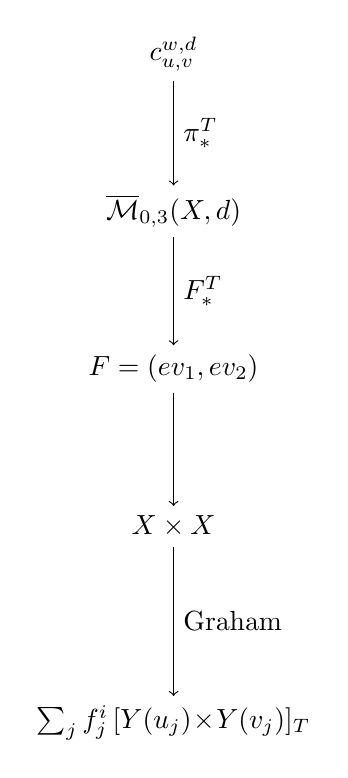
\begin{tikzpicture}[node distance=2cm, auto]
\node (EQLR) {$c_{u,v}^{w,d}$};
\node (M) [below of=EQLR] {$\overline{\mathcal{M}}_{0,3}(X,d)$};
\node (F) [below of=M] {$F=(ev_1,ev_2)$};
\node (XX) [below of=F] {$X\times X$};
\node (Graham) [below of=XX,yshift=-0.5cm] {$\sum_j f_j^i\,[Y(u_j)\!\times\!Y(v_j)]_T$};

\draw[->] (EQLR) -- (M) node[midway,right] {$\pi_*^T$};
\draw[->] (M) -- (F) node[midway,right] {$F_*^T$};
\draw[->] (F) -- (XX);
\draw[->] (XX) -- (Graham) node[midway,right] {Graham};
\end{tikzpicture}
\end{center}

\textbf{关键洞察}：量子上同调（quantum cohomology）中的曲线计数问题可以通过投影公式归约为 $X \times X$ 上的经典问题。这与 \cref{chap:TriplePositivity} 中三重 Schubert positivity 的证明策略形成了呼应——两者都使用了投影公式作为核心工具，将复杂几何对象分解为已知的 Schubert 基底的组合。

\section{与三重 Schubert Positivity 的联系}
\label{sec:ConnectionToTripleCh4}

在 \cref{chap:TriplePositivity} 中，我们遇到了 Refined Graham Positivity——Gao-Xiong 证明了三重变量 $(\mathbf{x}; \mathbf{y}; \mathbf{t})$ 下的展开系数 $c^w_{u,v}(\mathbf{y}, \mathbf{t})$ 是关于 $t_i - y_j$ 的非负多项式（\cref{def:RefinedGraham}）。Mihalcea 的结果与此有着深刻的联系。

\textbf{三重 Schubert Positivity}（triple Schubert positivity）涉及的是点的相交（point intersection），而等变量子上同调涉及的是曲线的计数（curve counting）。

\subsection{为什么这两个正性定理是相关的？}

粗略一看，三重 Schubert calculus 和等变量子上同调似乎是不同的领域：前者涉及多组变量，后者涉及量子修正。但它们都关注 Schubert 结构系数的正性，而且都涉及旗流形的几何。

当我们仔细审视时会发现：\textbf{两者都反映了旗流形中 Schubert 簇相交理论的基本非负性}。在三重情形，这种非负性来自点的相交；在量子情形，它来自曲线的计数。数学工具不同，但几何本质相同。

\subsection{旗流形情形的联系}

当 $X = Fl_n = GL_n/B$ 时，等变量子上同调的 Equivariant Quantum Littlewood-Richardson 系数 $c_{u,v}^{w,d}$ 与三重 Schubert calculus 中的正性有如下关系：

取特殊情形 $d = 0$（无量子修正），$c_{u,v}^{w,0}$ 正好是经典等变上同调（equivariant cohomology）的系数——即 Graham 的结果（\cref{def:GrahamPositivity}）。此时，Equivariant Quantum Littlewood-Richardson 系数的正性退化为 Graham positivity。

当考虑量子修正 $d \neq 0$ 时，新的正性结果补充了 \cref{chap:TriplePositivity} 的框架。几何上，这是因为量子上同调涉及曲线的计数，而三重情形只涉及点。\textbf{关键区别}在于：三重 Schubert positivity 涉及的是点的相交（point intersection），而等变量子上同调涉及的是曲线的计数（curve counting）。

\subsection{另一种 torus 作用：$T'$-等变版本}

Mihalcea 论文的第 7 节还讨论了另一种 torus 作用下的正性——$T' = (\mathbb{C}^\times)^m$ 作用在旗簇上。这种情形与 \cref{chap:TriplePositivity} 中的三重变量理论更加接近。

\subsubsection{$T'$ 的构造}

设 $X = PGL(m)/P$ 是部分旗流形。$T' = (\mathbb{C}^\times)^m$ 通过以下方式作用在 $X$ 上：

对 $t' \in T'$ 和 $x \in X$，
$$t' \cdot x = \varphi(t') x,$$
其中 $\varphi: (\mathbb{C}^\times)^m \to (\mathbb{C}^\times)^m / \mathbb{C}^\times \cong T$ 是商态射。

\textbf{注意}：$T$ 是 $PGL(m)$ 的极大环面，而 $T'$ 是更大的 torus。两者的关系是 $T = T'/\mathbb{C}^\times$。

\subsubsection{$T'$-等变上同调的坐标}

在 $T'$-等变上同调中，$H_{T'}^*(pt) = \mathbb{Z}[T_1, \ldots, T_m]$，其中每个 $T_j$ 是某个 $\mathbb{P}^n$ 上 $\mathcal{O}(1)$ 丛的第一陈类。

\subsubsection{从 $T$ 到 $T'$ 的变量变换}

关键事实是：$T$-等变量子上同调中的负单根 $x_j$（对应字符 $z_{j+1}/z_j$）在 $T'$-等变版本中变为 $T_j - T_{j+1}$。

\begin{Corollary}[$T'$-等变量子上同调 Positivity {\cite[Corollary 7.1]{Mihalcea}}]
\label{cor:TdashPositivity}
在 $T'$-等变量子上同调中，Equivariant Quantum Littlewood-Richardson 系数是关于变量 $T_1 - T_2, \ldots, T_{m-1} - T_m$ 的非负系数多项式。
\end{Corollary}

\textbf{与三重 positivity 的联系}：这与 Graham 在 \cite{knutson2005} 中研究的 Grassmannian 情形一致。这里，正性涉及的是差值 $T_i - T_j$，这与三重 positivity 中的 $t_i - y_j$ 结构惊人地相似——两者都涉及同类变量之间的差值。

\textbf{几何直觉}：$T_j - T_{j+1}$ 测量的是旗流形上相邻坐标的相对位置。这种相对坐标的选择是自然的，因为绝对值在物理上不可观测量（只有相对差值才有意义）。

\section{几何意义}
\label{sec:GeometricMeaningCh4}

我们已经看到了 Theorem \cref{th:EQCPositivity} 的代数陈述。但从几何角度理解，这个定理告诉我们什么？

\subsection{Gromov-Witten 不变量的正性}

Equivariant Quantum Littlewood-Richardson 系数 $c_{u,v}^{w,d}$ 是（3 点，带基点，亏格 0）Gromov-Witten 不变量（Gromov-Witten invariant）\footnote{定义见 \cite[Definition 1.2]{Mihalcea}（亦见 \cref{def:GromovWittenClass}）。问：什么是 Gromov-Witten 不变量？它计数的是什么？见附录 \cref{sec:GW-invariant}。}：
$$c_{u,v}^{w,d} = \langle \sigma(u), \sigma(v), \widetilde{\sigma}(w) \rangle_{0,3,d}.$$

它计数的是满足以下条件的稳定映射（stable map）$f: \mathbb{P}^1 \to X$ 的个数 \cite[Example 1.2.1]{FultonQuntum1997}：
\begin{itemize}
\item $f$ 的像代表同调类 $d \in H_2(X, \mathbb{Z})$；
\item $f(p_1) \in g_1 X(u)$，$f(p_2) \in g_2 X(v)$，$f(p_3) \in g_3 Y(w)$（其中 $g_i \in G$ 是一般位置，general position）。
\end{itemize}
其中 $p_1, p_2, p_3$ 是 $\mathbb{P}^1$ 上的三个标记点（marked points）。

从纯粹的几何角度，这些计数自然是非负的——计数``有多少条曲线通过指定位置''这个问题，答案显然不能是负数。

而 Theorem \cref{th:EQCPositivity} 进一步指出：\textbf{即使加入了等变修正（这会产生关于 $x_i$ 的多项式因子），整体系数仍然保持非负}。

\textbf{为什么这不显然？} 在等变上同调（equivariant cohomology）中，类不再是子簇的直接上同调类，而是提升到 $X \times_T ET$（即 $X$ 关于 torus 作用的同伦商空间/homotopy quotient）上的类。在这种更抽象的设置中，上同调类的相交理论变得复杂——我们不再能简单地说``两条子簇相交于几个点``，因为相交的结果可能是一个上同调类，而不是一个数字。在这种更抽象的设置中，非负性不再能从几何相交直接读出。Mihalcea 的证明揭示了隐藏的统一结构。

\subsection{与其他正性结果的比较}

在 Schubert calculus 的研究中，有多种不同层次的正性 \cite{knutson2003,FultonQuntum1997}。它们之间存在包含关系：

\begin{enumerate}
\item \textbf{经典 LR 系数}（classical LR coefficient）：$c_{u,v}^w \in \mathbb{N}$，计数交点个数——最直接的正性；
\item \textbf{Graham positivity}：$c_{u,v}^w \in \mathbb{Z}[x_i]$，等变修正的多项式系数非负——经典情形的等变推广；
\item \textbf{三重 positivity}（\cref{chap:TriplePositivity}）：$c_{u,v}^w(\mathbf{y}, \mathbf{t}) \in \mathbb{N}[t_i - y_j]$，多组变量情形；
\item \textbf{Mihalcea positivity}（本章）：$c_{u,v}^{w,d} \in \mathbb{Z}[x_i]$，量子版本同样正。
\end{enumerate}

这些正性之间存在蕴含关系：
$$c_{u,v}^w \in \mathbb{N} \Longrightarrow c_{u,v}^w \in \mathbb{Z}[x_i] \Longrightarrow c_{u,v}^{w,d} \in \mathbb{Z}[x_i].$$

每一代的正性都包含了前一代作为特殊情形（取特定的退化参数）。这种``稳定性''不是显然的——它反映了 Schubert calculus 核心结构的深层不变性。

\section{本章小结}
\label{sec:Chapter4Summary}

本章我们跟随 Mihalcea 的工作，探索了等变量子上同调中的正性问题。让我们回顾一下这段旅程的脉络：

\textbf{问题的起源}：从经典 Schubert calculus 到等变上同调（equivariant cohomology），Graham 证明了 Peterson 猜想——等变系数仍然满足正性。一个自然的问题是：这个性质能否推广到量子上同调？

\textbf{核心突破}（Mihalcea, 2007）：答案是肯定的。等变量子上同调的结构常数 $c_{u,v}^{w,d}$ 仍然是关于负根 $x_i$ 的非负整数系数多项式。

关键要点如下：
\begin{enumerate}
\item \textbf{Peterson 猜想的历史}：由 Peterson 提出（1997），由 Graham 证明（2001），Mihalcea 将其推广到量子情形（2007）——这是一段跨越十年的数学探索；
\item \textbf{等变量子上同调} $QH_T^*(X)$ 是等变上同调（equivariant cohomology）和量子上同调（quantum cohomology）的共同推广，同时包含了这两者的结构；
\item \textbf{主定理}（Theorem \cref{th:EQCPositivity}）：Equivariant Quantum Littlewood-Richardson 系数 $c_{u,v}^{w,d}$ 是关于负根 $x_i$ 的非负整数系数多项式；
\item \textbf{证明策略}：通过 projection formula 将 Equivariant Quantum Littlewood-Richardson 系数的计算归约到 $X \times X$ 上的问题，然后应用 Graham positivity——这是一种精巧的归约思想；
\item \textbf{与 \cref{chap:TriplePositivity} 的联系}：三重 positivity 涉及点的相交，而量子上同调涉及曲线的计数，两者都满足正性——不同的数学工具，相同的深层结构；
\item \textbf{几何意义}：正性反映了 Gromov-Witten 不变量的内在非负性——即使在等变量子上同调的抽象设置中，几何直觉仍然成立。
\end{enumerate}

这一结果与 Chapter 1 的 Gao-Xiong 三重 positivity 工作以及 Chapter 3 的量子 Schubert 多项式理论共同构成了现代 Schubert calculus 的核心框架。

在下一章中，我们将继续探索 Schubert calculus 的其他方面，包括量子版本的更多应用。

% === 用户问答记录 ===
% （暂无）

\section{附录：Equivariant Quantum Littlewood-Richardson 系数正性证明详解}
\label{sec:appendix-eqc-proof}

\subsection{背景（Background）}

本节给出 Theorem \cref{th:EQCPositivity} 的详细证明思路。该定理由 Mihalcea 在 2007 年证明，是量子 Schubert calculus 的里程碑结果。

证明的核心思想是将 Equivariant Quantum Littlewood-Richardson 系数的计算归约到 Graham 的经典 positivity 定理（Theorem \cref{th:GrahamPositivity}）。

\subsection{参数定义（Parameter Definitions）}
\begin{itemize}
\item $X = G/P$：齐次空间（homogeneous space）
\item $B = T \cdot U$：Borel 子群（Borel subgroup），其中 $U$ 为幂幺根基（unipotent radical）\footnote{问：在 Borel 子群分解 $B = T \cdot U$ 中，$U$ 称为``幂幺根基``，这是什么意思？见附录 \cref{sec:unipotent-radical}。}
\item $B^- = w_0 B w_0$：相反 Borel 子群（opposite Borel subgroup）
\item $B' = T \cdot (U^- \times U^-)$：半直积（semidirect product）
\item $\overline{\mathcal{M}} = \overline{\mathcal{M}}_{0,3}(X,d)$：稳定映射模空间（stable map moduli space）
\item $ev_i : \overline{\mathcal{M}} \to X$：评估映射（evaluation map）
\item $F = (ev_1, ev_2) : \overline{\mathcal{M}} \to X \times X$
\item $\Lambda = H_T^*(pt) = \mathbb{Z}[x_1, \ldots, x_r]$
\end{itemize}

\subsection{已知条件（Given）}

\begin{Corollary}[Graham Positivity on $X \times X$ {\cite[Corollary 6.2]{Mihalcea}}]
\label{cor:GrahamOnXX}
设 $V \subset X \times X$ 为 $T$-稳定子簇，则在 $H_T^*(X \times X)$ 中
$$[V]_T = \sum_i f_i [Y(u_i) \times Y(v_i)]_T,$$
其中 $f_i \in \Lambda = \mathbb{Z}[x_1,\ldots,x_r]$ 是非负系数多项式。
\end{Corollary}

\begin{Lemma}[Lemma 6.1 — 映射 $F$ 的构造 {\cite[Lemma 6.1]{Mihalcea}}]
\label{prop:Lemma61F}
设 $X = G/P$ 是旗流形，$T$ 是最大环面。定义映射
$$F = (ev_1, ev_2) : \overline{\mathcal{M}}_{3}(X, d) \to X \times X,$$
这是 $T$-等变且适当的（proper）映射。对于每个 $w \in W^P$，$F^{-1}(X(u) \times Y(v))$ 是 $T$-稳定的。
\end{Lemma}

\begin{Lemma}[Lemma 6.4 — $ev_3^{-1}(Y(w))$ 的不可约分支 {\cite[Lemma 6.4]{Mihalcea}}]
\label{prop:ev3inverse}
设 $v \in W^P$，则 $ev_3^{-1}(Y(v))$ 是 $T$-stable、reduced、不可约分支（irreducible component）的不交并，每个分支的余维数为 $l(v)$。
\end{Lemma}

\begin{Lemma}[Lemma 6.3 — Kleiman Transversality {\cite[Lemma 6.3]{Mihalcea}}]
\label{prop:KleimanTransversality}
设 $Z$ 是不可约 $G$-簇，$F: Z \to X \times X$ 是 $G$-等变映射（$G$ 在 $X \times X$ 上对角作用），则对任意 $u, v \in W^P$，$F^{-1}(X(u) \times Y(v))$ 是 reduced、locally irreducible 的，其余维数为 $c(u) + l(v)$。
\end{Lemma}

\textbf{Projection Formula}（\cite[(1)]{Mihalcea}）：对于 $T$-等变映射 $f: X_1 \to X_2$，
$$f_*^T\left((f^T)^*(a) \cdot b\right) = a \cdot f_*^T(b).$$

\textbf{Lemma 2.3 — 等变 Poincaré 对偶}（\cite[Lemma 2.3]{Mihalcea}）：
对于任意 $u, v \in W^P$，有
$$\langle \sigma(u)^T, \sigma(v)^T \rangle_T = \delta_{u,v},$$
其中 $\langle \cdot, \cdot \rangle_T$ 是 $H_T^*(X)$ 上的等变 Poincaré pairing。
\label{prop:Lemma23Poincare}

\textbf{Push-Forward Formula}（\cite[(2)]{Mihalcea}）：对于纤维积图（fiber product diagram），
$$f_*([V]) = \sum_i m_i a_i [f(V_i)],$$
其中 $V_i$ 是原像的不可约分支（irreducible component）。

\textbf{等变 Poincaré对偶}（\cite[Proposition 3.1]{Mihalcea}）：
$$\langle \sigma(u)^T, \widetilde{\sigma}(v)^T \rangle_T = \delta_{u,v}.$$
这里 $\widetilde{\sigma}(v)^T$ 表示 equivariant quantum Schubert class。

\subsection{目标（Goal）}

证明 Equivariant Quantum Littlewood-Richardson 系数
$$c_{u,v}^{w,d} = \pi_*^T\left((ev_1^T)^* \sigma(u)^T \cdot (ev_2^T)^* \sigma(v)^T \cdot (ev_3^T)^* \widetilde{\sigma}(w)^T\right)$$
是关于 $x_i$ 的非负系数多项式。

\subsection{详细推导步骤（Derivation Steps）——对应论文 \S 6}

\textbf{步骤 1：引入映射 $F$（对应 \cref{prop:Lemma61F}，\cite[Lemma 6.1]{Mihalcea}）。}

定义 $F = (ev_1, ev_2) : \overline{\mathcal{M}} \to X \times X$，这是 $T$-等变且适当的（proper）映射。

由 \cref{prop:ev3inverse}（\cite[Lemma 6.4]{Mihalcea}），$ev_3^{-1}(Y(w))$ 是 $T$-稳定、约化、不可约分支（irreducible component）的不交并，每个分支余维数为 $l(w)$。

利用 $ev_1^* \sigma(u)^T \cdot ev_2^* \sigma(v)^T = (F^T)^*[X(u) \times X(v)]_T$，可将表达式重写为
$$c_{u,v}^{w,d} = (\pi_{X \times X})_*^T F_*^T\left((F^T)^*[X(u) \times X(v)]_T \cdot (ev_3^T)^* \widetilde{\sigma}(w)^T\right).$$

\textbf{步骤 2：应用 Projection Formula（对应 \cite[Eq.\ (1)]{Mihalcea}）。}

由 projection formula，
$$F_*^T\left((F^T)^*[X(u) \times X(v)]_T \cdot (ev_3^T)^* \widetilde{\sigma}(w)^T\right) = [X(u) \times X(v)]_T \cdot F_*^T\left((ev_3^T)^* \widetilde{\sigma}(w)^T\right).$$

\textbf{步骤 3：处理 $ev_3$ 的原像。}

由 \cref{prop:ev3inverse}（\cite[Lemma 6.4]{Mihalcea}），$ev_3^{-1}(Y(w))$ 是 $T$-稳定、约化、不可约分支 $V_i$ 的不交并，每个分支余维数为 $l(w)$。

应用 push-forward formula（对应 \cite[Eq.\ (2)]{Mihalcea}）：
$$F_*^T\left((ev_3^T)^*[Y(w)]_T\right) = \sum_i a_i [F(V_i)]_T,$$
其中 $a_i$ 是映射 $F|_{V_i} : V_i \to F(V_i)$ 的次数（degree）。

因此，
$$c_{u,v}^{w,d} = \sum_i a_i (\pi_{X \times X})_*^T\left([X(u) \times X(v)]_T \cdot [F(V_i)]_T\right).$$

\textbf{步骤 4：应用 Graham Positivity。}

对每个 $[F(V_i)]_T$，由 Graham 定理（\cite[Corollary 6.2]{Mihalcea}），
$$[F(V_i)]_T = \sum_j f_j^i [Y(u_j) \times Y(v_j)]_T,$$
其中 $f_j^i \in \Lambda$ 是非负系数多项式。

代入并使用 projection formula：
{\small
\begin{align*}
&(\pi_{X \times X})_*^T\left([X(u) \times X(v)]_T \cdot [Y(u_j) \times Y(v_j)]_T\right) \\
&= (\pi_{X \times X})_*^T\big((pr_1^T)^* \sigma(u)^T \cdot (pr_2^T)^* \sigma(v)^T \\
&\quad\cdot [Y(u_j) \times Y(v_j)]_T\big) \\
&= \langle \sigma(u)^T, \widetilde{\sigma}(v_j)^T \rangle_T \cdot \delta_{v,v_j} \\
&= \delta_{u,u_j} \cdot \delta_{v,v_j}.
\end{align*}}

其中第二个等式来自 \cref{prop:Lemma23Poincare}（\cite[Lemma 2.3]{Mihalcea}），第三个等式来自等变 Poincaré对偶（equivariant Poincaré duality）。

\textbf{步骤 5：得到最终表达式。}

综合步骤 3 和 4，
$$c_{u,v}^{w,d} = \sum_i a_i \sum_j f_j^i \cdot \delta_{u,u_j} \cdot \delta_{v,v_j}.$$

由于所有 $a_i \in \mathbb{N}$（次数），所有 $f_j^i \in \Lambda$ 是非负多项式，我们得出结论：$c_{u,v}^{w,d}$ 是关于 $x_1, \ldots, x_r$ 的非负整数系数多项式。

这完成了 Theorem \cref{th:EQCPositivity} 的证明。

\subsection{关键洞察（Key Insight）}

整个证明的核心洞察是：\textbf{量子上同调（quantum cohomology）中的曲线计数问题可以通过 projection formula（投影公式）归约为 $X \times X$ 上的经典问题}。

为什么这个归约是可能的？因为 $c_{u,v}^{w,d}$ 的定义涉及三个评估映射（evaluation maps）$ev_1, ev_2, ev_3$。通过适当组合前两个映射 $F = (ev_1, ev_2)$，我们将问题从 $\overline{\mathcal{M}}$ 推送到 $X \times X$。在 $X \times X$ 上，Graham positivity 已经告诉我们任何 $T$-稳定子簇的类都可以写成非负多项式系数的线性组合。

\textbf{这个证明的深层意义}在于：它表明即使在量子上同调中引入了新的复杂度（stable map moduli space，稳定映射模空间；curve counting，曲线计数），最终的正性结果仍然来自于经典几何中的简单事实。这种``复杂性中的简单性''是数学之美的体现。

\endinput
